\begin{figure}[H]
    \centering
    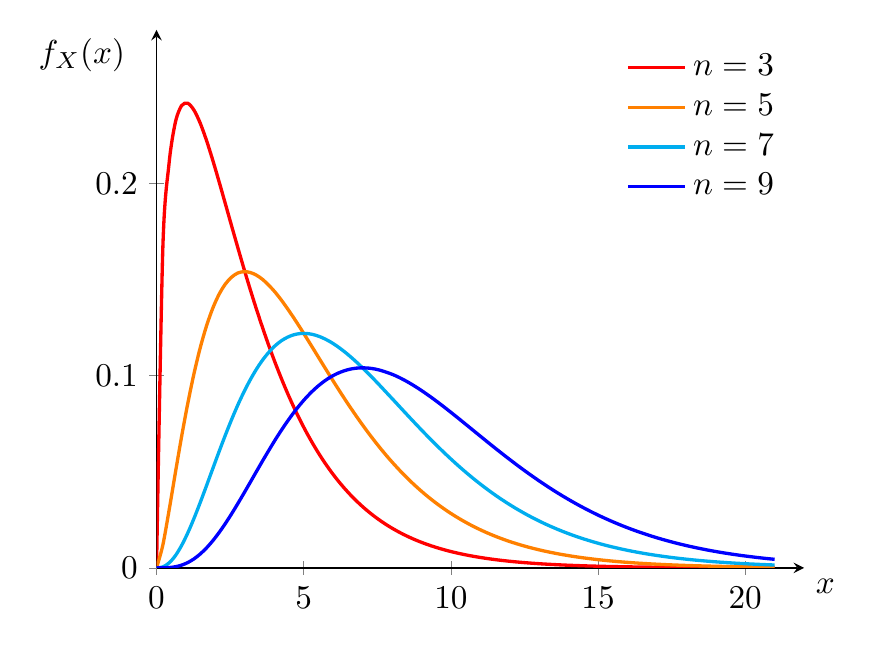
\begin{tikzpicture}[
        declare function={gamma(\z) = (2.506628274631*sqrt(1/\z) + 0.20888568*(1/\z)^(1.5) + 0.00870357*(1/\z)^(2.5) - (174.2106599*(1/\z)^(3.5))/25920 - (715.6423511*(1/\z)^(4.5))/1244160) * exp((-ln(1/\z)-1)*\z);},
        declare function={gammapdf(\x,\k) = \x^(\k-1)*exp(-\x/2) / (2^\k*gamma(\k));},
        scale=1.2
    ]
        \begin{axis}[
            axis lines=left,
            xmax=22,
            ymax=0.28,
            xtick={0,5,10,15,20},
            xticklabels={0,5,10,15,20},
            ytick={0, 0.1, 0.2},
            yticklabels={0, 0.1, 0.2},
            xlabel=$x$,
            ylabel=$f_X(x)$,
            xlabel style={at={(axis description cs:1,0)},anchor=north west},
            ylabel style={at={(axis description cs:-0.2,0.9)},anchor=south west,rotate=-90},
            samples=100,
            legend entries={$n=3$, $n=5$, $n=7$, $n=9$},
            legend style={draw=none}
        ]
            \addplot [smooth, domain=0:21, red, line width=1] {gammapdf(x,1.5)};
            \addplot [smooth, domain=0:21, orange, line width=1] {gammapdf(x,2.5)};
            \addplot [smooth, domain=0:21, cyan, line width=1] {gammapdf(x,3.5)};
            \addplot [smooth, domain=0:21, blue, line width=1] {gammapdf(x,4.5)};
        \end{axis}
    \end{tikzpicture}
\end{figure}